\chapter{トランスポート層(その2) UDP}

本書の解説では、UDPを一番最後に廻しました。これは、UDPは簡単なプロトコルですが、インターネットプロトコル層のパケット通信そのままです。プロトコル自体はものすごく簡単なのですが、インターネットプロトコル層の知識なしでは、理解がむずかいという落とし穴があります。

そんな理由で、本書の締めくくりはUDPの開設となります。

\section{UDPとはどんなプロトコルか}

トランスポート層の実際のプロトコルとして、ポートによる経路多重化と、疑似ヘッダによるエラーチェックだけ行うUDP(User Datagram Protocol)について説明しよう。UDPは、データ送信の前にコネクションをはる動作がない。そのため、UDPによる通信を、コネクションレス型と言うことがある。

また、その名の通り、インターネットプロトコル層のデータグラムを、そのままトランスポート層経由で使用できるようにしたもの、と考えることもできる。相手にデータを届けるという観点で見たUDPの基本動作は、ポートによる経路多重化が付加されただけで、インターネットプロトコル層と変わらない。

\section{UDPヘッダ}

UDPは、送信元ポート、宛先ポート、データ長、チェックサムからなる、8オクテットのヘッダを持つ。
データ長のフィールドが2オクテットなので、UDPデータグラムの最大の大きさは、64KiBとなる。また、最小の大きさは、ヘッダだけの8オクテットである。

IPv4では、インターネットプロトコル層のデータの大きさが最大64KiBであり、更にネットワークアクセス層が一度に送出できるデータの大きさははそれより小さいことが多いため、最大の大きさで送信されることは少ない。

\begin{figure}[htbp]
	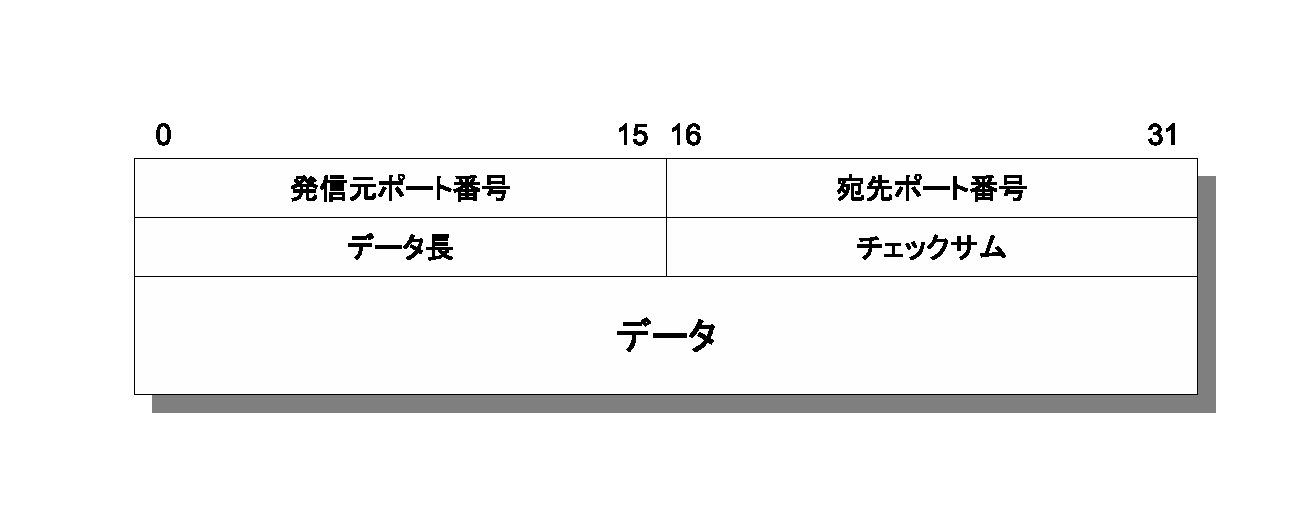
\includegraphics[width=12cm,clip]{draw/udpdatagram.eps}
	\caption{UDPデータグラムの構造}
	\label{fig:udpdatagram}
\end{figure}

\subsection{IPv6ジャンボグラム対応}
インターネットプロトコル層にIPv4を用いる場合、UDPでは、64KiBを越えるデータをひとつのデータグラムで送信することはできない。これは、IPv4のデータグラムのサイズの上限が、UDPのデータグラムのサイズの上限となるためである。

後ほど改めて説明するが、IPv6では、最大4GiBまでのデータをひとつのデータグラムで送信することができる。この拡張を、IPv4ジャンボグラムという。そのため、IPv6ジャンボグラムを提案したRFC2675の中で、UDPのデータサイズの拡張も定義されている。

インターネットプロトコル層にIPv6を使用しており、64kibを越えるデータを送信するときは、UDPヘッダのサイズフィールドを0にする。この値は、レガシーなUDPでは決して現れない値である。

もしサイズフィールドが0であるUDPヘッダを受信したら、到達したデータのサイズをそのUDPデータグラムのサイズとする。疑似ヘッダによるチェックサム計算には、その実際のサイズをパラメータとして、使用する。

\section{UDPによる通信}

UDPによる通信は、通信前の準備や、データの到達確認などは行われない。オプションとして、チェックサムによるデータグラムの破損チェックがあるくらいである。このように、一見すると信頼性がないプロトコルは、どのような使い方をするのだろうか。

UDPは、エンドツーエンドのコネクションをはるコストに対して、通信の量が少ないプロトコルの場合に使用される。例えば、データグラム一つに収まる質問に対して、データグラム一つに収まる解答を返せば終了するプロトコルが該当する。

また、クライアントから送られるデータをただ記録するだけの場合にも使用される。どのような場合かというと、データの流れが基本的に一方向で、エンドツーエンドでの対話がほぼ存在しない場合などである。

前者の例として、代表的なアプリケーション層のプロトコルがDNSであり、後者の例がsyslogやSNMPである。

身も蓋もなく言えば、CPUやネットワークの貧弱であった時代に、TCPほど確実な通信でなくていいところは、通信に必要なリソースの少ないUDPで済ませていた。また、当時の計算機やネットワークでTCPを使うとデータを取りこぼしかねなかった、重いアプリケーションが、UDPを使用していた。\footnote{そのため、近年はUDPを使用していたデータロガーをTCPを使用して実装し直す例がある。例えば、syslogの置き換えアプリとして、TCPを用いるsyslog-ngが挙げられる。}

また、IP電話や音声や動画のストリームのように、発信元に対して応答確認をする時間や、データの到着順の管理などが再生時のラグに繋がるサービスについても、UDPが使用される。もっとも、チェックサムによる破損チェックを有効にしていた場合、データの破損したUDPデータグラムは破棄される。そのため、UDPさえ使えばストリーミングは滞りなく流れるわけではない。


\section{UDPの実装}
ここまで説明したUDPの動作で気がついたかもしれないが、UDPの受信時の動作とは、インターネットプロトコルによって届いたデータグラム卯を、UDPヘッダに記載されたポート番号で特定されるアプリケーションのインタフェイスに届けることである。

また、送信時も、UDPデータグラムをIPでカプセル化して送信するだけである。トランスポート層のUDPとしての制御は全く入らない。

そのため、UDPのプロトコルスタックのコードは、IPのプロトコルスタックのコードのなかに実装されることが多い。

\section{UDPの疑似ヘッダ}

\begin{figure}[htbp]
	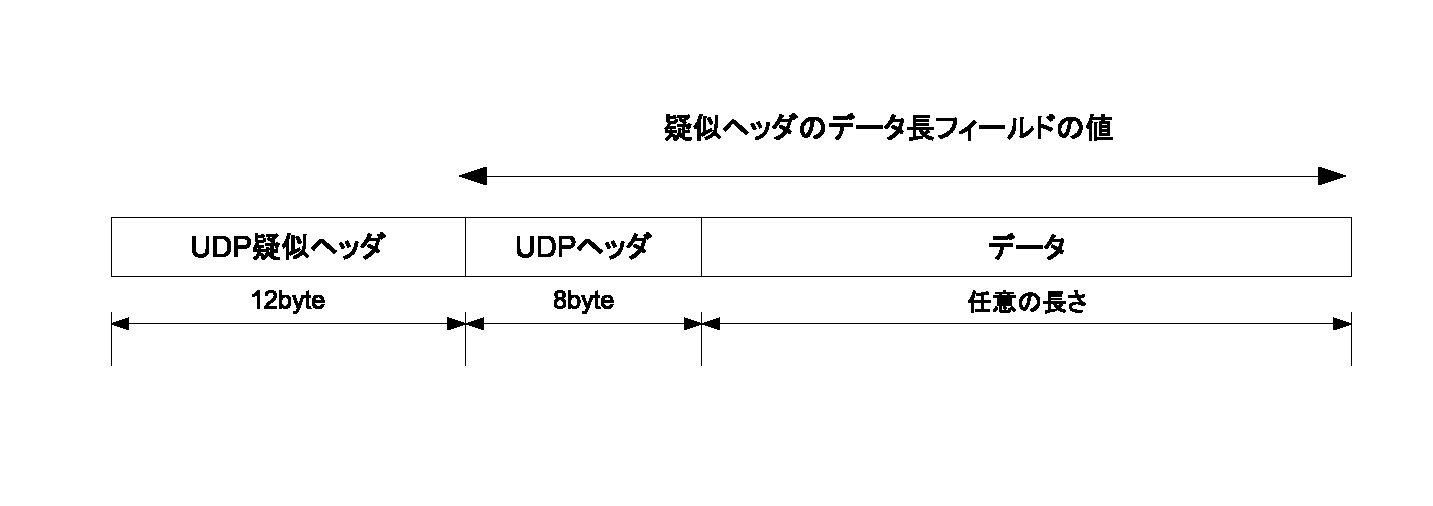
\includegraphics[width=12cm,clip]{draw/udppseudoheader.eps}
	\caption{UDP疑似ヘッダを含めたUDPデータグラム}
	\label{fig:udppseudoheader}
\end{figure}


UDPは、図\ref{fig:udppseudoheader}のように、疑似ヘッダがUDPヘッダの前にあることにして、到着したデータグラムの正当性を検証する。

UDP 疑似ヘッダは、IPデータグラムのヘッダを簡略化したものである。UDP疑似ヘッダは発信元と宛先のIPアドレスの情報を含む。それによって、UDPは誤った経路で送られたデータグラムを破棄する。また、チェックサムを計算するときは、UDPデータグラムの先頭に疑似ヘッダがあるものとして計算を行う。

UDPヘッダのチェックサムフィールドの値は、疑似ヘッダ込みで計算された値となる。


算出されたチェックサムが0であれば、UDPヘッダのチェックサムフィールドは0xFFFF(1の補数演算)として送出される。これは、0に対して、1の補数を取った値となる。また、UDPヘッダのチェックサムフィールドが0x0000である場合は、送信側がチェックサムを生成しなかったということを意味する。送信側がチェックサムを生成しなかった場合、UDPはチェックサムによるデータグラムの正当性検査を行わない。

UDPでは、インターネットプロトコル層にIPv4を用い、上位プロトコルで、データ破損が問題とならない場合や、デバッグ中などは、チェックサム生成とチェックサムによる検査を省略することが許されている。これは、IPv4に、チェックサムによるデータの検証機能があることによる。

一方、インターネットプロトコル層にIPv6を用いるときは、チェックサムによる検証が必須となる。これは、IPv6では、データグラムの検証が省略されたからとなる。IPv6では、データの検証はトランスポート層のサービスとして定義された。



\subsection*{}
\begin{itembox}[l]{いもうとコラム UDP-Lite}

トランスポート層のプロトコルとして、UDPを更に緩くしたUDP-Liteというプロトコルがあります。
このUDP-Liteは、音声や動画向けを想定したトランスポート層のプロトコルです。

UDPとの違いは、音声や動画データの、ビット化けなどの軽微なデータ破損は、アプリケーション層における、デコード時の補正・補完で対応することを前提としていることです。つまり、アプリケーション層でデータの復元をを行う前提で、データグラムの到達を優先させるのがUDP-Liteというプロトコルです。

UDP-Liteは、UDPヘッダでのデータ長フィールドをチェックサム適用範囲(先頭から何オクテットまでのチェックサムを取るか)に変更しています。チェックサムによるデータの検証を行うときは、チェックサム適用範囲までのデータで計算します。
つまり、UDP-Liteでは、チェックサム適用範囲外のデータが壊れていても気にしません。

UDP-Liteは、UDPのサブセットでなくUDPと全く別の、トランスポート層のプロトコルとして実装されてます。


\end{itembox}



